\section{Why output length changes the comparison}
\label{sec:laws}

Standard AR decoding adds one token at a time, reusing its key-value (KV)
cache of earlier computation. DG refines positions together inside each
canvas and generates canvases sequentially. Its encoder caches input
context while its decoder refines the active canvas~\cite{diffusiongemma}.
Parallel output positions therefore do not mean all generation work
happens at once.

\begin{center}
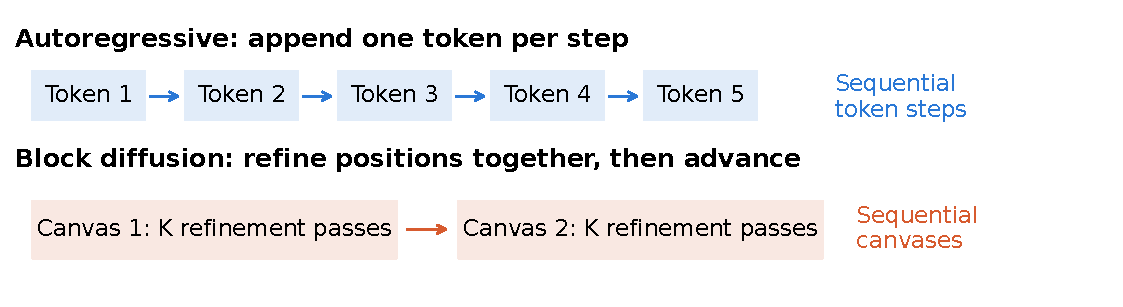
\includegraphics[width=.94\linewidth]{figures/decoding_schematic.pdf}
\captionof*{figure}{Decoding schedules (schematic). AR advances token by
token; DG refines each canvas over $K$ passes before starting the next.
These are execution patterns, not a timing scale.}
\end{center}

At a fixed prompt and decoding configuration, we estimate service time
$\widehat T$ in milliseconds by
\begin{align}
\label{eq:ar}
\widehat T_A(L) &= a_A+b_A L,\\
\label{eq:dg}
\widehat T_D(N_C) &= a_D+s_D(N_C-1),\qquad N_C\geq1.
\end{align}
Here $L$ is the generated token count and $N_C$ the number of decoded
canvases. The coefficients and units are listed below.

\begin{center}
\begin{tabular}{@{}llr@{}}
\toprule
Coefficient & Meaning & Fitted value \\
\midrule
$a_A$ & AR starting cost & \arBase\,ms \\
$b_A$ & AR incremental cost & \arSlope\,ms/token \\
$a_D$ & DG first-canvas cost & \dgBase\,ms \\
$s_D$ & DG additional-canvas cost & \dgStep\,ms \\
\bottomrule
\end{tabular}
\end{center}

Within the first canvas, the predicted times are equal at
\begin{equation}
\label{eq:lcross}
L^*=\frac{a_D-a_A}{b_A}
=\frac{\dgBase-\arBase}{\arSlope}\approx\crossoverL\quad\text{tokens}.
\end{equation}
The numerator is the difference in starting costs; dividing by AR's cost
per token gives the crossover length. Beyond this point, the model predicts
a diffusion advantage within the first canvas. Further canvases add cost,
so the comparison must be recalculated at each boundary.

This explains why longer required output can favor diffusion, but the
measured range matters. The AR fit covers only about 32--126 generated
tokens and uses mean times, whereas DG canvas costs summarize medians.
A fitted crossover is an approximate cost comparison, not proof of a
valid record or equal-quality speedup. Raising a maximum output budget
does not lengthen a response that has already reached its end-of-sequence
(EOS) stopping token. Appendix~\ref{app:secondary} gives a compact
budget-accounting example and supporting measurements.
